\newpage
\chapter{Traditional Sketching}
\label{sec:traditional}

Sketching is the traditional method for early-phase design when both
problems and solutions are unclear. Whereas some might view design as
a process that begins with a fixed problem definition and progresses
by optimization within constraints to refine the problem solution, to
others, the practice of design is as much a matter of
\textit{defining} the problem as \textit{solving} it.

Sketching enables people to work with abstract and uncertain elements,
interpreting and re-interpreting marks on the page that may be
ambiguous or hold alternative contending semantics. Sketched figures,
pictures and maps help people to focus their thoughts or to explain
ideas to others~\cite{do-design-sketches-tools}.

We talk about different kinds of renderings: artistic sketches, study
sketches, drawings, diagrams, schematics, blueprints, and so
on. Although the boundaries are not always clear, each is
characterized by the means of production, the kind of information it
communicates, and the role it plays in problem-solving.

Sketches support quick, informal information processing. We may write
a phone number on the whiteboard near our desk rather than typing. Or,
we may choose to make quick calculations or ``To-Do'' lists on a sheet
of paper because they are portable and easy to make. In his
book \textit{How to Solve It}, George Polya recommends drawing figures
to help understand and solve problems in
mathematics~\cite{polya-solve}. Sketches help us to visualize and
restructure problems to make solutions more readily apparent. For
example, the drawings in Figure \ref{fig:types-of-sketches} were made
by practitioners in different domains. Each depiction helps designers
to think about problems or possible solutions.

There is still a gap between what we know about how and why people
sketch and what kinds of things we can do to support it
computationally. To provide a basis for discussing computational
support we first survey the design and cognitive aspects
of \textit{traditional} sketching done with physical media.

\begin{figure}
\begin{center}

\subfigure[Project management diagram showing task precedence 
           of two projects. Hastily drawn boxes and arrows represent
           abstract activities.]  {

    \label{fig:sketch-type-pm}
    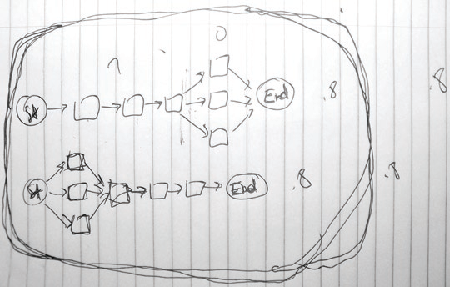
\includegraphics[width=0.42\linewidth]
      {img/sketch-type-project-management.pdf}
}
\hspace{0.03\linewidth}
\subfigure[An architect's floor plan sketch. It includes text, 
           spatial information, and symbols representing household
           items like a piano or dining table.] {

    \label{fig:sketch-type-architecture}
    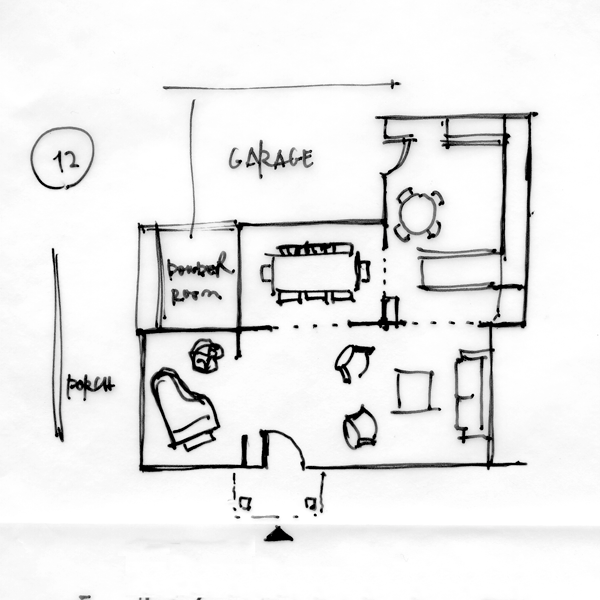
\includegraphics[width=0.42\linewidth]
      {img/sketch-type-architecture.pdf}
}
\caption{Sketches vary in domain and in the visual characteristics of marks.}
\label{fig:types-of-sketches}

\end{center}
\end{figure}

\section{Sketching in design}
\label{sec:traditional-in-design}

While designing, we iteratively explore and refine the problem
definition and proposed solutions. Sketching supports this creative
search process. We set out on our design task with some high-level
goals. However, due to the
ill-structured~\cite{simon-ill-structured-problems} and ``wicked''
nature of design~\cite{rittel-wicked}, we encounter unforeseen
opportunities and constraints as designing progresses. Those
opportunities and constraints may be implicit in the original problem
description, but designers expose them as they explore. The
discoveries are incorporated into the understanding of the problem and
potential solutions. Design problems are ``not the sort of problems or
puzzles that provide all the necessary and sufficient information for
their solution~\cite{cross-nature-nurture}.'' So it goes with
sketching. We draw different views of our model, which allows us to
perceive the problem in new ways.

Designers engage in a sort of ``conversation'' with their sketches in
a tight cycle of drawing, understanding, and
interpreting~\cite{schon-kinds-of-seeing}. Goldschmidt describes this
as switching between two reasoning modes: ``seeing that'' and ``seeing
as''~\cite{goldschmidt-dialectics}. Seeing \textit{that} is the
process of recognizing the literal, descriptive properties of the
drawing.  Seeing \textit{as} is figurative and transformative,
allowing the designer to re-interpret parts of the sketch in different
ways. For example, a designer may draw a sofa and see that the wood
constituting the back rest and the rear supports come into contact. In
this way the designer can see how the two parts could be redesigned as
one. The designer may be able to extract more information from the
sketch than is consciously put into it~\cite{goldschmidt-backtalk}.

Care must be taken to support this reflection when making design
software that employs sketch recognition. If the system interprets
drawings too aggressively or at the wrong time, it may prevent the
human designer from seeing alternative meanings; recognize too little
and the software is no better than paper. This is discussed further in
Sections \ref{sec:recognition-when}
and \ref{sec:recognition-how-much}.

Expertise plays a role in sketching as well. Design students begin to
sketch from the first day. Proficiency in sketching goes beyond
applying marks to the page---one must also interpret and re-interpret
drawings in order to use them effectively. Suwa and Tversky studied
differences between student and professional architects, finding that
professionals had greater skill in transformative
reasoning~\cite{suwa-analysis-students}. Buxton points out the
importance of recognizing the disparity between sketchers who can
expertly \textit{see as} and \textit{see that}, and those who can
not~\cite[page 118]{buxton-sketching}. Trained designers skillfully
examine the content from multiple perspectives, extracting different
interpretations.

Experimental and observational evidence suggest that people of
comparable skill use consistent methods when making drawings. This
consistency applies to the motor action of
drawing~\cite{van-sommers-cognition} and to higher-level semantic
notation. For example, the type of an architectural drawing
(e.g. floor plan, elevation, bubble diagram) can be discerned by
identifying particular visual elements the designer
employs~\cite{neiman-sketch-retrospective,do-design-sketches-tools}.

\section{Prototyping and fidelity}
\label{sec:traditional-prototyping}

Newman and Landay conducted ethnographies of web designers, focusing
on the use of informal design
techniques~\cite{newman-web-designers}. The designers were observed
making models in various media (such as on paper or with a computer)
at various levels of fidelity. Designers always sketch at the
beginning of a web design project, exploring numerous high-level
options. Frequently this early sketching phase is accompanied with
construction of low-fidelity prototypes made on paper or with
Microsoft
PowerPoint\texttrademark~\cite{arnowitz-software-prototyping}. As the
design progresses and designers begin making incremental edits, they
move to higher fidelity models. Client meetings are an important
forcing function in web design projects. When meeting with clients,
designers want to show polished prototypes produced with computer
software. Therefore designers used electronic tools earlier in the
process than they would otherwise have preferred.

Today most software tools support incremental refinement and
specification of details but do not adequately support idea generation
or exploration~\cite{terry-creative-ui}. Designers who begin using
software tools in the early phases of design tend to make superficial
explorations of possible solutions. Further, because tools are poor
for exploration but good for specifying details (font, line weight,
and color), designers tend to focus on nuances that are not yet
important. Observing that current tools are inadequate for creative
pursuits, researchers have developed calligraphic tools such as SILK
and DENIM, which aim to support the early phases of
design~\cite{landay-silk,lin-denim}.

Paper sketches dominate the early phases of design as people generate
new ideas, in a process Goel terms ``lateral
transformations''~\cite{goel-sketches-of-thought}. But as soon as the
web designer believes he or she will make incremental revisions (which
Goel calls ``vertical transformations'') they switch to a computer
tool.

It is not always best to use high-fidelity models for testing
designs. Walker and Takayama observed web site developers performing
usability tests of ongoing interface designs. They found that
high-fidelity, computer-based models are not significantly better than
low-fidelity, paper-based models when testing design
ideas~\cite{walker-fidelity}. This finding supports the conventional
wisdom that inexpensive and quickly made low-fidelity prototypes are
appropriate in iterative design, building, and testing.

\section{Sketches as a symbol system}

\begin{figure}
  \centering
  \subfigure[Overloaded semantics: The cloud and tree have similar
             shapes but different meanings due to context.] {
    \label{fig:cloud-1} 
    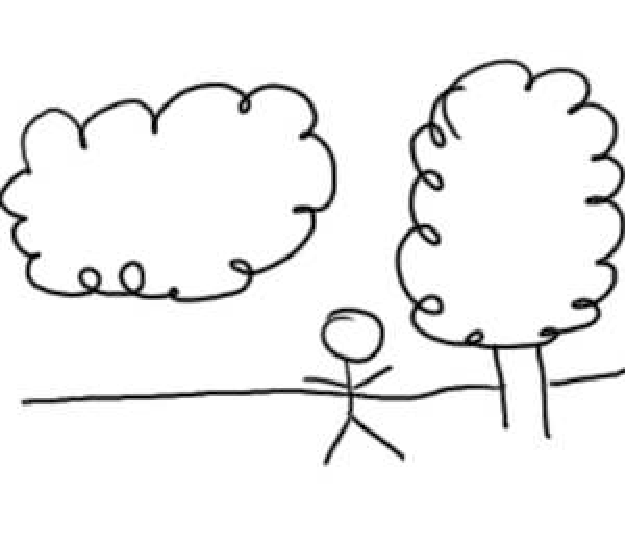
\includegraphics[width=0.25\linewidth]{img/cloud-1.pdf} 
  }
  \hspace{0.03\linewidth}
  \subfigure[Ambiguity: Changing the drawing slightly changes our
             interpretation. The object on the left may be a cloud, or
             it may be a cartoon thought bubble.] { 
    \label{fig:cloud-2} 
    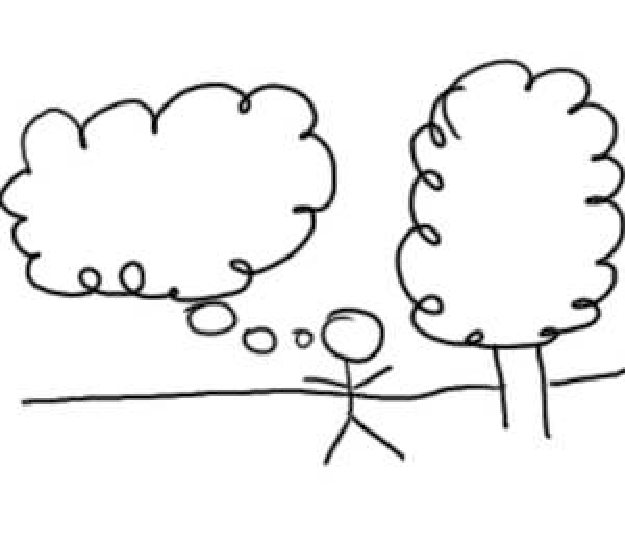
\includegraphics[width=0.25\linewidth]{img/cloud-2.pdf} 
  }
  \hspace{0.03\linewidth}
  \subfigure[Additional information helps us reason about the intended
             identity of elements. Text inside the cloud indicates it
             is a cartoon thought bubble.]  {
    \label{fig:cloud-3} 
    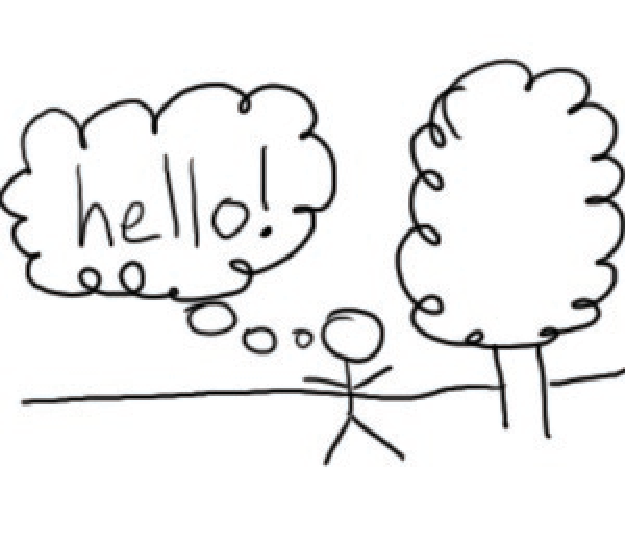
\includegraphics[width=0.25\linewidth]{img/cloud-3.pdf} 
  }
  \caption{Overloaded semantics and ambiguity.}
  \label{fig:cloud}
\end{figure}

Goodman provides a comprehensive framework for analyzing the
properties of various symbol systems, including
sketches~\cite{goodman-symbols}. Goel places sketching in Goodman's
framework, noting that sketches have \textit{overloaded semantics},
they are \textit{ambiguous}, \textit{dense},
and \textit{replete}~\cite{goel-sketches-of-thought}. These properties
describe one particular sense of sketching in which the drawer's marks
may be idiosyncratic.

Sketches have ``overloaded semantics'': The same symbol may mean
different things depending on context. Further, a sketched symbol may
be ``ambiguous'', meaning that the symbol affords more than one
plausible interpretation.  Figure~\ref{fig:cloud} illustrates these
properties. A lumpy shape can be used to indicate many things
including clouds, trees, or thought bubbles. We interpret the shape
differently depending on context.

Sketched symbols are ``dense'', indicating there is a continuous range
between instances of the same symbol. While there may be minute visual
discrepancies between symbol instances, Goel claims that such symbols
are also ``replete'': no aspect of the sketched symbol may be safely
ignored (Figure~\ref{fig:dense-replete}).

The pen strokes constituting a sketch serve various functions. Ink may
indicate abstract domain symbols (e.g. diode, treble clef), object
boundaries, actions (e.g. arrows indicating containment or movement),
dimensions and units, annotations, region texturing, and so on. Some
parts of a sketch are more dense and replete than others. For example
a diode's properties do not change if it is drawn with a slightly
larger triangle. However, subtle variations in how a desk lamp is
drawn might lead to substantially different aesthetic responses to it.

\begin{figure}
\begin{center}
  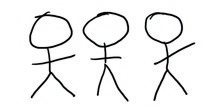
\includegraphics[angle=0, origin=c,
  width=3.5cm]{img/dense-replete-stick-figures.pdf}

  \caption{Different instances of the same stick figure vary along a
  continuum (\textit{dense}). However, the visual properties of
  individual symbols may (or may not) communicate additional
  information (\textit{replete}). Is the figure at the right waving? }

  \label{fig:dense-replete}
\end{center}
\end{figure}

Gross and Do discuss some properties of hand-drawn diagrams from the
perspective of building tools to support design drawing
activities~\cite{gross-ecn-uist}. The authors distinguish sketches
from diagrams, noting that diagrams are ``composed of primitive
elements chosen from a small universe of simple symbols---boxes,
circles, blobs, lines, arrows.'' This list is certainly not
exhaustive, but it does illustrate the general idea that diagrams have
a limited vocabulary. In practice, sketches and diagrams from various
dialects may be combined (e.g. mathematical notation on the same page
as circuit diagrams and hand written notes.)

Freehand diagrammatic drawings are abstract, ambiguous, and
imprecise. \textit{Abstract} symbols denote elements whose identities
or properties are not (yet) important or known. For example,
Figure~\ref{fig:sketch-type-pm} on page \pageref{fig:sketch-type-pm}
shows a project management diagram of two hypothetical projects. The
activities composing each project are abstract---they could represent
anything. The value of the sketch is that it shows the project's
network topology and does not draw attention to what the specific
activities are. 

An \textit{ambiguous} symbol has many plausible interpretations. The
floor plan sketch in Figure~\ref{fig:sketch-type-architecture} shows
several rectangles indicating rooms, furniture, shelves, or
counters. Human observers can confidently disambiguate the intended
meaning of some rectangles, but others remain unclear. The
bottom-right of the sketch shows two armchairs and a sofa with an
ambiguous rectangle in the middle that could plausibly represent
either a rug or a coffee table.

Last, freehand diagrams are \textit{imprecise}. Imprecision allows
designers to work with rough values (e.g. ``about two meters wide'')
and avoid premature commitment. Imprecision also indicates that the
design is by no means final.

The notational properties of sketches make them powerful tools for
supporting visual thinking. Designers may leverage ambiguities in
their sketches to see new meanings, for example. However, these same
properties present challenges for accurate software recognition.

The degree to which a drawing is ambiguous, imprecise, and abstract
varies among instances, and people might interpret them differently. A
rough sketch is useful to designers, especially for brainstorming and
incremental development of ideas. But in order for the sketch to be
transformed into a finished product (e.g. for manufacturing), it must
be made unequivocal, precise, and concrete. The process of moving from
the informal sketch to the formal specification involves drawings that
are semi-ambiguous, partially precise, and with some abstractions
given definite identities.

\section{Cognitive and mechanical aspects of drawing}
\label{sec:traditional-cognitive-mechanical}

Larkin and Simon compared \textit{diagrammatic} notation
with \textit{sentential} (written or spoken) systems, suggesting that
spatial notation often affords more efficient information processing
than an equivalent written
statement~\cite{larkin-diagrams}. \textit{Efficiency} of information
processing refers to how much computation is necessary to translate
input into understanding. For example, we may state the relationship
between supply and demand in a market economy with a mathematical
(sentential) description as in
Figure~\ref{fig:markets-sentential}. Market equilibrium is found where
the values of supply and demand intersect. In a sentential
representation, we must calculate to find equilibrium. However, given
a graph (diagrammatic) as in Figure~\ref{fig:markets-diagrammatic}, we
directly see where the supply and demand curves intersect and
immediately read the associated values. Even though the
representations provide equivalent information, the diagrammatic form
can be more efficient, depending on the viewer's goals.

\begin{figure}
  \centering
  \subfigure[Written (sentential) form.] { 
    \label{fig:markets-sentential} 
    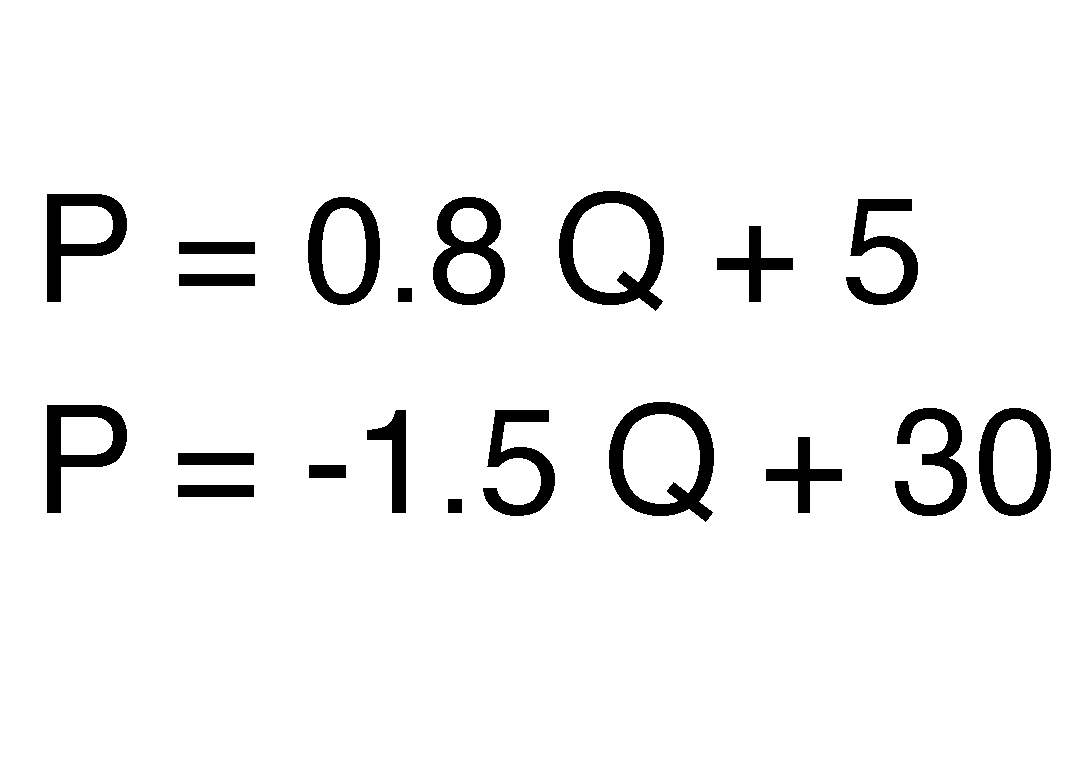
\includegraphics[width=2in]{img/market-eqn.pdf} 
  }
  \hspace{0.5cm}
  \subfigure[Graphic (diagrammatic) form.] {
    \label{fig:markets-diagrammatic} 
    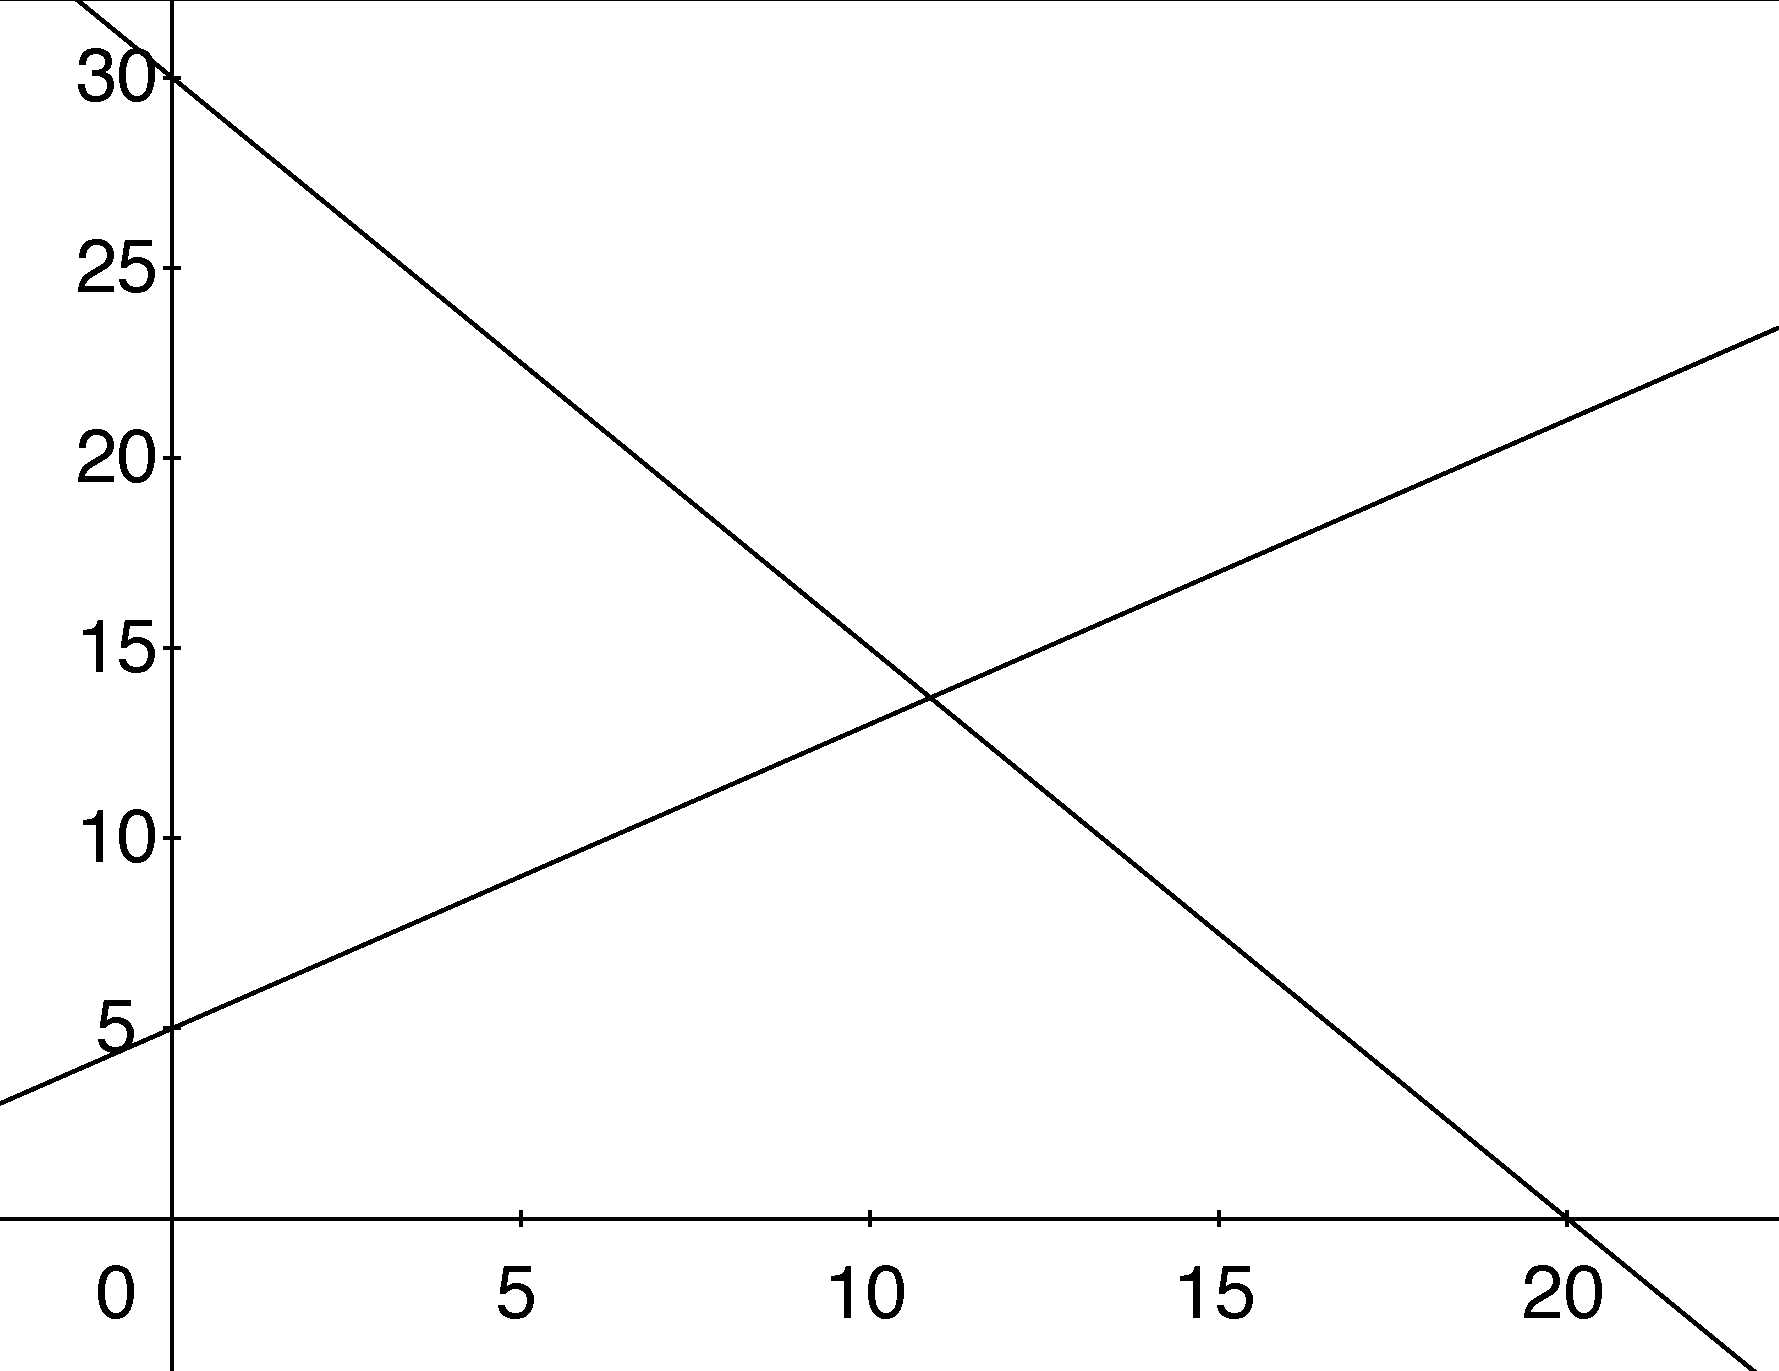
\includegraphics[width=2in]{img/market-graph.pdf}
  }
  \caption{Sentential and diagrammatic representations of supply and
  demand provide equivalent information.}
  \label{fig:markets}
\end{figure}

When people sketch, they ``incorporate relevant information and omit
the irrelevant''~\cite{tversky-sketching-thinking}. Drawing allows
people to use paper as external storage, reducing and augmenting
cognitive load. Diagrammatic notation schematizes domain
information~\cite{tversky-diagrammatic-communication}. Hand-drawn
route maps, for example, are usually made with a simple visual
vocabulary consisting of rectangles or circles indicating buildings,
lines or arcs representing paths, and junctions where paths
intersect~\cite{tversky-routes}. The shape and curvature of buildings
and paths is drawn approximately. Given a well-drawn map, humans have
little trouble reconciling differences between the map and the
physical world it represents.

Spatial representations offer a powerful means for learning in many
domains. Sketching allows learners to represent concepts as they
understand them, and allows more experienced people to spot
inconsistencies or areas where additional learning is
needed~\cite{forbus-cogsketch-tutorial}.

Van Sommers extensively studied how people
draw~\cite{van-sommers-cognition}. This includes the mechanics of
using one's arm, wrist, hand, and fingers when drawing. His research
examines the effects of culture, handedness, and expertise on how
drawings are made. He found that of the many possible ways of making a
drawing, subjects tended to use consistent strategies. For example,
subjects were asked to trace over short lines scattered about a large
sheet of paper. The lines did not overlap and represented the full
range of rotations. Right-handed drawers had a strong tendency to draw
from left to right and top to bottom. Left-handers also showed the
tendency to draw top to bottom but showed a slight preference towards
drawing right to left.

Sezgin gives a compelling example of consistent stroke
ordering~\cite{sezgin-phd-thesis}. Participants were asked to draw
common objects such as the stick figure shown in
Figure~\ref{fig:stick-figure} thirty or more times. This stick figure
has six components: the head, a torso, two arms, two legs. The lines
can be drawn in 720 distinct sequences \nohyphens{($6!=720$)}.
However, participants used only about five of those component
orderings to draw the figure. Further, each participant showed a
strong individual bias to draw the symbol using the same sequence
(e.g. head, torso, legs, and finally the arms).

\begin{figure}
\begin{center}
  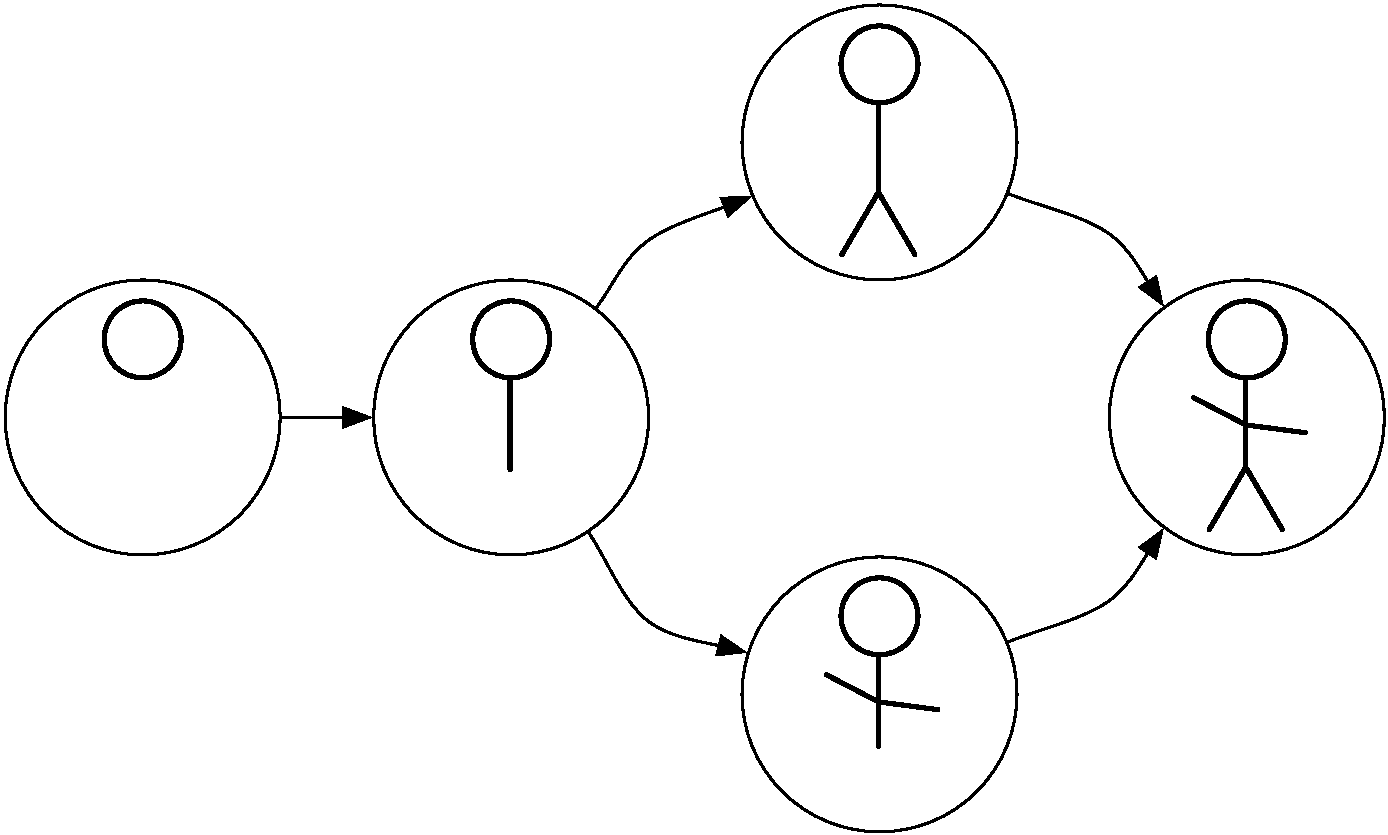
\includegraphics[width=2.5in]{img/sezgin-sketching-style-diagram.pdf} 

  \caption{A stick figure with six components can be drawn in any one
  of 720 possible orders, but only about five are used in
  practice \protect~\cite{sezgin-phd-thesis}. Two of those orders are
  shown in this sketching style diagram.}

\label{fig:stick-figure}
\end{center}
\end{figure}

A drawer's preferred direction of making strokes depends on the
semantics of whatever is being drawn. Van Sommers shows that although
people will choose to draw arbitrary lines according to a preference
(largely determined by handedness), people will deviate from those
preferences when drawing things that hold meaning. Participants were
asked to draw common things, including a rake and cigarette smoke. We
know from experience that a rake is held at the top with the rake's
fingers contacting the ground. Cigarette smoke rises. Van Sommers'
participants generally drew the rake from top to bottom, but the smoke
from bottom to top. He posits this is because our knowledge of an
object's properties informs the way we draw it.

Stroke ordering can also be affected by perceptual properties of a
drawing, even if the drawing's meaning is not clear.  Van Sommers
asked experiment participants to trace over the picture in
Figure~\ref{fig:grape-clusters}. Each ``grape'' in a cluster has a
boundary. The number represents the mean position in the drawing
sequence. The grape ``on top'' is usually drawn first, with
neighboring grapes drawn next.

Van Sommers uses the term \textit{anchoring} to explain the sequence
that some strokes are made. Anchoring is an example of a control
strategy for making marks. The grape ``on top'' serves as a convenient
anchor for drawing its neighbors. It is easier to control the start
and end locations of a mark if there is already something to attach it
to. Another control strategy for making marks
is \textit{containment}. In depictions with a structure enclosing
something else (such as a bowl of fruit), the container is typically
drawn first. Anchoring and containment may be useful control
strategies for improving sketch recognition efficiency.

\begin{figure}
  \begin{center}
  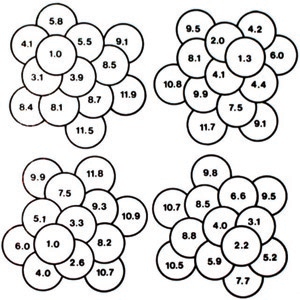
\includegraphics[width=2in]{img/van-sommers-grapes.pdf}
  \caption{``Grape Clusters'' drawn by right-handed participants in
    van Sommers' study showing the mean position in the drawing
    sequence.}
  \label{fig:grape-clusters} 
  \end{center}
\end{figure}

Some researchers have noted the prominent place of sketching in design
and have studied sketching as a tool. A series of experiments by Goel
looked at the cognitive affordances of
sketching~\cite{goel-sketches-of-thought}. These studies compared
traditional pencil-and-paper sketching with sketches made with a
computer drawing application. Participating designers were asked to
design an artifact using either a software paint program or using
pencil and paper. The software tool was modified to only support
structured input such as straight lines, rectangles, and ellipses. He
found that the structured notation system (computer application) did
not afford the same level of rapid exploration of design ideas as
using an unstructured system (pencil-and-paper freehand
sketching). Sketching supports designers in easily trying many ideas,
which Goel calls \textit{lateral transformations}. This is
distinguished from \textit{vertical transformations}, characterized by
refining ideas rather than exploring new ones.

The transformation types identified by Goel correspond to the
activities done at different stages of design described by Newman and
Landay~\cite{newman-web-designers}. Early in the design process
designers are concerned with idea generation and exploration (lateral
transformations). Later on designers make iterative revisions and
refinement (vertical transformations). The goal of many computational
sketching tools is to support lateral transformations.


\section{Summary: traditional sketching and computation}
\label{ref:traditional-summary}

If we hope to effectively support sketching with computation, we must
first understand the practical aspects of traditional sketching. 

Sketching is an important---perhaps necessary---tool for doing
design. It gives us a way to quickly make provisional drawings, which
help us efficiently make sense of spatial, relational
information. Sketches let us make marks that are as vague or specific
as we need. Because sketched elements can easily be ambiguous, rough
drawings afford different interpretations. We may therefore reflect on
our sketches and see new meaning in existing marks. People sketch in
part because they don't know exactly what they are making---sketching
facilitates exploration.

Low-fidelity prototypes are especially important as tools to test
ideas during early design. This is because they are easy to make,
allowing designers to quickly expose problems before committing to
decisions. Sketching is a common method of creating such prototypes.

In order for computers to recognize sketches, we must develop
techniques to transform imprecisely made marks into discrete
symbols. However, some of the properties that make a sketch useful for
a human (overloaded semantics, ambiguous, imprecise, etc.) complicate
the task of computer recognition.

We can make use of consistencies in how people draw to inform
recognition. First, we observe that some kinds of sketches are made
using restricted visual vocabulary, e.g., diagrams of electronic
circuits or web page layouts. Second, consistencies in the mechanical
act of drawing (such as anchoring and containment) can be used to
further guide recognition. For example, recalling
Figure~\ref{fig:stick-figure} we know that people are likely to use
only a small number of ways to draw a stick figure even though there
are hundreds of possible stroke orderings. This can help make
recognition strategies more efficient by utilizing commonly used
patterns before less frequently used ones.
